%==============================================================================
%== template for LATEX poster =================================================
%==============================================================================
%
%--A0 beamer slide-------------------------------------------------------------
\documentclass[final]{beamer}\usepackage{graphicx, color}
%% maxwidth is the original width if it is less than linewidth
%% otherwise use linewidth (to make sure the graphics do not exceed the margin)
\makeatletter
\def\maxwidth{ %
  \ifdim\Gin@nat@width>\linewidth
    \linewidth
  \else
    \Gin@nat@width
  \fi
}
\makeatother

\definecolor{fgcolor}{rgb}{0.2, 0.2, 0.2}
\newcommand{\hlnumber}[1]{\textcolor[rgb]{0,0,0}{#1}}%
\newcommand{\hlfunctioncall}[1]{\textcolor[rgb]{0.501960784313725,0,0.329411764705882}{\textbf{#1}}}%
\newcommand{\hlstring}[1]{\textcolor[rgb]{0.6,0.6,1}{#1}}%
\newcommand{\hlkeyword}[1]{\textcolor[rgb]{0,0,0}{\textbf{#1}}}%
\newcommand{\hlargument}[1]{\textcolor[rgb]{0.690196078431373,0.250980392156863,0.0196078431372549}{#1}}%
\newcommand{\hlcomment}[1]{\textcolor[rgb]{0.180392156862745,0.6,0.341176470588235}{#1}}%
\newcommand{\hlroxygencomment}[1]{\textcolor[rgb]{0.43921568627451,0.47843137254902,0.701960784313725}{#1}}%
\newcommand{\hlformalargs}[1]{\textcolor[rgb]{0.690196078431373,0.250980392156863,0.0196078431372549}{#1}}%
\newcommand{\hleqformalargs}[1]{\textcolor[rgb]{0.690196078431373,0.250980392156863,0.0196078431372549}{#1}}%
\newcommand{\hlassignement}[1]{\textcolor[rgb]{0,0,0}{\textbf{#1}}}%
\newcommand{\hlpackage}[1]{\textcolor[rgb]{0.588235294117647,0.709803921568627,0.145098039215686}{#1}}%
\newcommand{\hlslot}[1]{\textit{#1}}%
\newcommand{\hlsymbol}[1]{\textcolor[rgb]{0,0,0}{#1}}%
\newcommand{\hlprompt}[1]{\textcolor[rgb]{0.2,0.2,0.2}{#1}}%

\usepackage{framed}
\makeatletter
\newenvironment{kframe}{%
 \def\at@end@of@kframe{}%
 \ifinner\ifhmode%
  \def\at@end@of@kframe{\end{minipage}}%
  \begin{minipage}{\columnwidth}%
 \fi\fi%
 \def\FrameCommand##1{\hskip\@totalleftmargin \hskip-\fboxsep
 \colorbox{shadecolor}{##1}\hskip-\fboxsep
     % There is no \\@totalrightmargin, so:
     \hskip-\linewidth \hskip-\@totalleftmargin \hskip\columnwidth}%
 \MakeFramed {\advance\hsize-\width
   \@totalleftmargin\z@ \linewidth\hsize
   \@setminipage}}%
 {\par\unskip\endMakeFramed%
 \at@end@of@kframe}
\makeatother

\definecolor{shadecolor}{rgb}{.97, .97, .97}
\definecolor{messagecolor}{rgb}{0, 0, 0}
\definecolor{warningcolor}{rgb}{1, 0, 1}
\definecolor{errorcolor}{rgb}{1, 0, 0}
\newenvironment{knitrout}{}{} % an empty environment to be redefined in TeX

\usepackage{alltt}\usepackage{graphicx, color}
%% maxwidth is the original width if it is less than linewidth
%% otherwise use linewidth (to make sure the graphics do not exceed the margin)
\makeatletter
\def\maxwidth{ %
  \ifdim\Gin@nat@width>\linewidth
    \linewidth
  \else
    \Gin@nat@width
  \fi
}
\makeatother


\usepackage{natbib}
\def\newblock{\hskip .11em plus .33em minus .07em} %for natbib and beamer 
\usepackage[orientation=landscape,size=a0,
            scale=1         % font scale factor
           ]{beamerposter}
           
\geometry{
  hmargin=2.5cm, % little modification of margins
}

%
%\usepackage{floatrow}

\usepackage{subfigure}
\usepackage[utf8]{inputenc}
%\usepackage{verbatim}
\usepackage{color}

\linespread{1.15}
%
%==The poster style============================================================
\usetheme{sharelatex}

%==Title, date and authors of the poster=======================================
\title
%[Super Conference, 1 - 10 July 2013, New York, USA] % Conference
{ % Poster title
Interactive 3 and 4D Images of High Resolution Neuroimage Data 
}

%\author{ % Authors
%John Muschelli\inst{1}, Elizabeth Sweeney\inst{1}, Ciprian Crainiceanu\inst{1}
%}
%\institute
%[Johns Hopkins Bloomberg School of Public Health] % General University
%{
%\inst{1} Johns Hopkins Bloomberg School of Public Health
%}
\author{ % Authors
John Muschelli, Elizabeth Sweeney, Ciprian Crainiceanu
}
\institute
[Johns Hopkins Bloomberg School of Public Health] % General University
{
Johns Hopkins Bloomberg School of Public Health
}
\date{\today}


\usepackage{hyperref}
\IfFileExists{upquote.sty}{\usepackage{upquote}}{}
\IfFileExists{upquote.sty}{\usepackage{upquote}}{}

\begin{document}
\begin{frame}[fragile]
%==============================================================================
\begin{multicols}{2}
%==============================================================================
%==The poster content==========================================================
%==============================================================================

\section{Introduction}

Most neuroimaging figures for publications/presentations commonly contain:
\begin{itemize}
\item 3 orthogonal slices (Figure~\ref{fig:ortho}, left) or lightbox views (Figure~\ref{fig:ortho}, right)
\begin{figure}
  \begin{minipage}[b]{3.5in}
    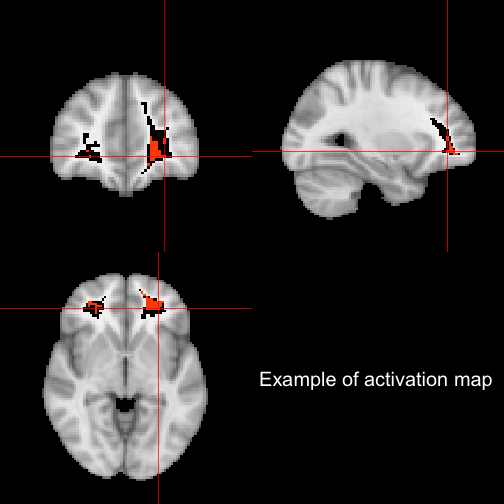
\includegraphics[width=7in, height=5in]{./figure/ortho.png}
  \end{minipage}\hfill
  \begin{minipage}[b]{3.5in}
    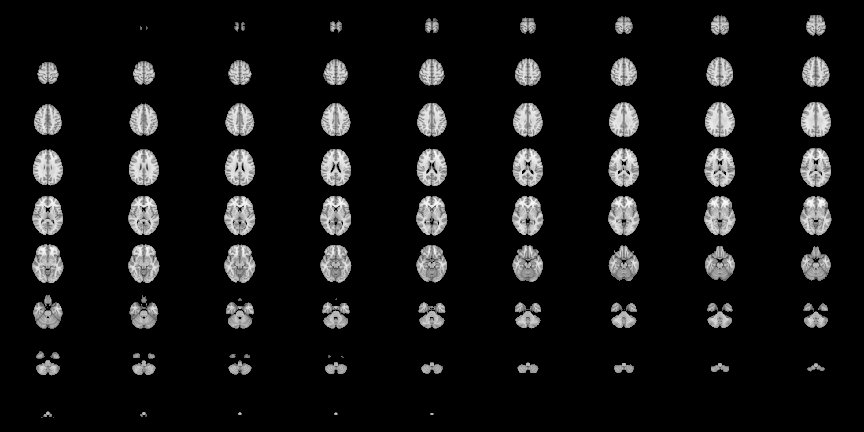
\includegraphics[width=7in, height=5in]{./figure/lightbox.png}
  \end{minipage}\hfill  
  \begin{minipage}[b]{7in}
    \caption{
		Example of an orthographic (left) representation of a 3D image or a lightbox (right) view of an image.  The orthographic view allows the user to see all 3 planes, but the choice of presentation can be arbitrary and sometimes misleading.  The lightbox view shows all slices, which is more comprehensive but more cumbersome; presenting condensed information in this format is more difficult.  3D images, using opacity and interactive controls, resolve both of these problems.
    } \label{fig:ortho}
  \end{minipage}
\end{figure}
\item 2D images of 3D rendering of surfaces (Figure~\ref{fig:others}, left panel).
\item ``Glass'' brain - maximum intensity projections (Figure~\ref{fig:others}, right panel).
\end{itemize}

\begin{figure}
  \begin{minipage}[b]{3.5in}
    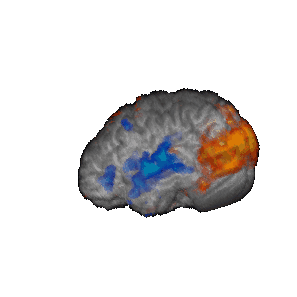
\includegraphics[width=7in, height=5in]{3d_proj.png}
  \end{minipage}\hfill
  \begin{minipage}[b]{3.5in}
    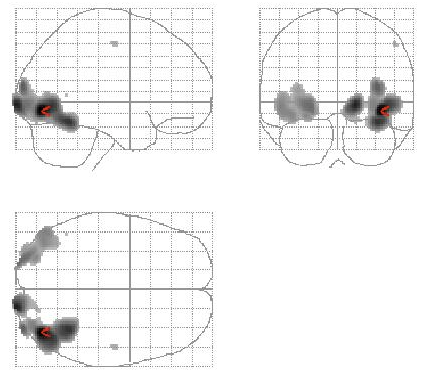
\includegraphics[width=7in, height=5in]{glass_brain.png}
  \end{minipage}\hfill  
  \begin{minipage}[b]{7in}
    \caption{
		Example of a 3D projection with overlaid colored activation (left) and a glass brain.  These both show different aspects of activation, but still do not adequately show where the activation is located in 3D space.  {\scriptsize Images from { \url{http://www2.fmrib.ox.ac.uk/education/fmri/images/trans_anim.gif}} and { \url{http://brainimaging.waisman.wisc.edu/~oakes/spm/visual_stim_demo/fmri_visual_stim.html}}, respectively.}
    }   \label{fig:others}
 \end{minipage}
\end{figure}


% pdf files (see below) or as
We recommend a set of software tools that allows to produce interactive 3D and 4D brain images using open-source software for presentations and publications. These images can be embedded into web-pages (\url{http://biostat.jhsph.edu/~jmuschel/webGL/index_jsed.html}), creating an interactive environment for the user/reader without any additional software. Examples of applications of these tools are: 1) observing a region of interest in a brain; 2) tracking the lesion formation process in the brain of a subject with multiple sclerosis; 3) describing the evolution of blot clot in the brain of a patient with a stroke. The methods and approaches can be much more generally applicable.

\section{Tools}
\texttt{R} (\href{http://cran.r-project.org/}{http://cran.r-project.org/}) is a statistical software that can analyze neuroimaging data.  RGL is an adapation of the open graphics library for \texttt{R} \cite{opengl}.  Using the \texttt{misc3d} and \texttt{rgl} packages, one can render interactive 3D brain images with regions of interest (ROIs) and using the \texttt{writeWebGL} function, can export them to webpages \citep{rgl, misc3d}.  Using this method also has the benefit that these are highly reproducible figures, and if preprocessing and analysis are done in \text{R}, the entire pipeline from preprocessing to 3D figures can be in one system.  
Other rendering systems exist such as 3D Slicer (\href{http://slicer.org/}{http://slicer.org/}), Paraview (\href{http://www.paraview.org/}{http://www.paraview.org/}), and Freesurfer (\href{https://surfer.nmr.mgh.harvard.edu/}{https://surfer.nmr.mgh.harvard.edu/}).  We chose to focus on \texttt{R} as this system has almost all the qualities we believe denotes a good figure, described below, and many other systems lack exportability to webpages. 

\section{What makes a good figure?}
For a 3D figure to be useful, it must have some characteristics that make it more useful than a 2D image.  It must allow the user to 
\begin{itemize}
\item Interact with the image such as rotation, translation, zooming
\item Display {\bf sub-surface} objects, eliminating projections on the cortical surface 
\item Render {\bf multiple surfaces} and contrast them with {\bf colors}
\item Made in a reproducible way so that reviewers can check validity and they can also easily be remade for future comparisons
\end{itemize}

We consider a 4D figure to be any 3D image with the above qualities, as well as the ability to change the structures/time points/ROIs being displayed.  The uses of such figures are observing fMRI activation over tasks/time, contrasting group activation maps, as in Figure~\ref{fig:fig2} (right panel) or looking at structural changes across groups or within a person over time.  For these interactive controls, we believe that webpages, online or standalone, are the most natural, capable and accessible media as the user/reader requires no third-party software for viewing.
\vfill
\columnbreak
 
\section{Why use \texttt{R}?}

\begin{itemize}
\item It is free.  (Download from \url{http://cran.r-project.org/})
\item Highly customizable: plot functions gives flexibility to the user to add or change figure characteristics
\item Multi-platform and a large user community
\item Has state-of-the-art statistical methods and a growing number of packages for neuroimaging analysis
\item Reproducibility: \texttt{knitr} and \texttt{Sweave} are tools that allow code and text to be ``weaved'' together.
\item Code can be ported for {\bf automated} figure creation (see below)
\end{itemize}




\subsection{Example R code}
Below we give example code to generate Figure~\ref{fig:fig2} (left).  Using such code in the future allows researchers to easily and quickly make new, customized 3D figures.
\begin{knitrout}
\definecolor{shadecolor}{rgb}{0.969, 0.969, 0.969}\color{fgcolor}\begin{kframe}
\begin{alltt}
tmp <- \hlfunctioncall{readNIfTI}(\hlstring{"MNI152_T1_2mm_brain.nii"}, reorient = FALSE)  \hlcomment{### read in brain image}
dtemp <- \hlfunctioncall{dim}(tmp)  \hlcomment{# get dimensions}
\hlfunctioncall{contour3d}(tmp, x = 1:dtemp[1], y = 1:dtemp[2], z = 1:dtemp[3], level = 4500, 
    alpha = 0.15)  \hlcomment{### make the surface object - RGL renders}
\hlfunctioncall{contour3d}(tmp, level = \hlfunctioncall{c}(8200, 8250), alpha = \hlfunctioncall{c}(0.5, 0.8), add = TRUE, color = \hlfunctioncall{c}(\hlstring{"yellow"}, 
    \hlstring{"red"}))  \hlcomment{### this would be the ``activation'' or surface you want to render}
\hlfunctioncall{text3d}(x = dtemp[1]/2, y = dtemp[2]/2, z = dtemp[3] * 0.98, text = \hlstring{"Top"})  \hlcomment{### add text}
\hlfunctioncall{text3d}(x = dtemp[1] * 0.98, y = dtemp[2]/2, z = dtemp[3]/2, text = \hlstring{"Right"})
\hlfunctioncall{writeWebGL_split}(dir = \hlfunctioncall{file.path}(outdir, \hlstring{"webGL"}), width = 700, height = 500, 
    template = \hlfunctioncall{file.path}(outdir, \hlstring{"my_template.html"}))  \hlcomment{### export this to a webpage}
\end{alltt}
\end{kframe}
\end{knitrout}


%\section{Possible Exports}
%Export types from RGL and 3D Slicer include OBJ, STL, PLY, and standalone WebGL embedded in html (RGL only) object types.   These types integrate with most 3D visualization systems. The X Toolkit (XTK: \url{goxtk.com}) is one Javascript system that use these to render interactive online webpages, and this format is used by 3D Slicer and can be used with RGL, see Figure~\ref{fig:fig2} (right).  We believe \texttt{R} has the some of the best qualities for this figure generation process.


\section{Result and discussions}

 
% \vskip1ex
%\begin{figure}
%\raggedleft
%  \begin{minipage}[c]{10in}
%    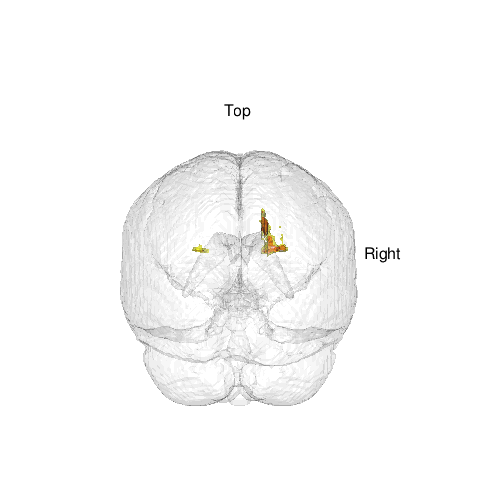
\includegraphics[height=4in]{snapshot.png}
%  \end{minipage}\hfill
%  \begin{minipage}[c]{10in}
%    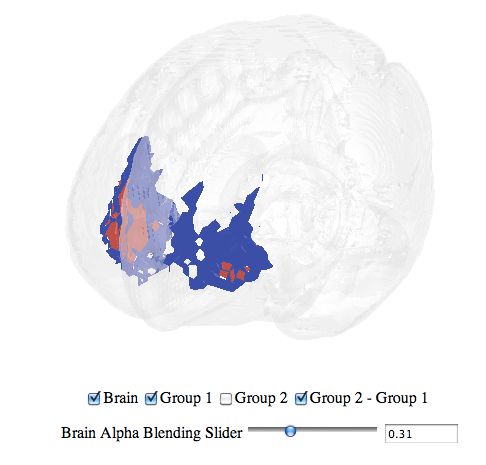
\includegraphics[width=3.5in, height=6in]{./figure/4D_snapshot2.png}
%  \end{minipage}\hfill  
%  \caption{An example of a 3D figure made completely in \texttt{R}}
%\end{figure}
%\vskip2ex

\begin{figure}
  \begin{minipage}[t]{3.5in}
    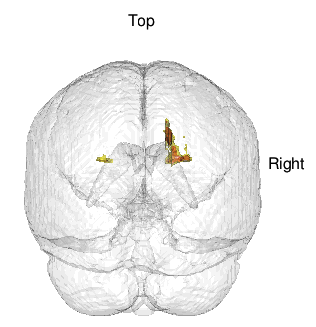
\includegraphics[width=6in, height=6in]{snapshot_crop.png}
  \end{minipage}\hfill
  \begin{minipage}[t]{3.5in}
    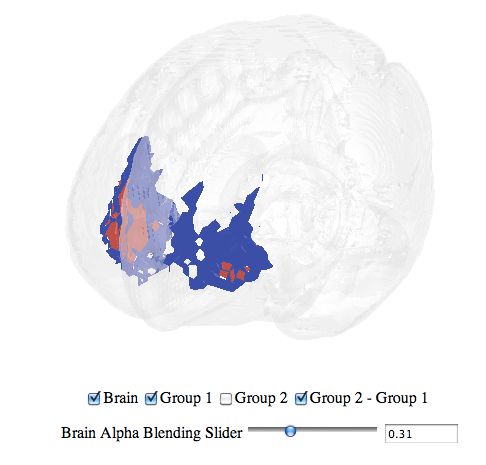
\includegraphics[width=6in, height=6in]{./figure/4D_snapshot2.png}
  \end{minipage} \hfill
  \begin{minipage}[b]{7in}
    \caption{
		Example of a 3D rendered image from RGL (left) using the \texttt{writeWebGL} function.  This was generated using the code above in a fully reproducible framework.  The right panel shows (in addition to some Javascript controls) how these can be made into 4D figures on webpages.  The checkboxes allow the user to switch between activation maps for each group, as well as the contrast.  The slider allows the user to change the opacity/transparency of the brain.  The combination of these simple controls can be used to navigate through many dimensions in 3D, such as contrasts or time.   }   \label{fig:fig2}	
 \end{minipage}
\end{figure}
 



\section{Conclusions}

Webpages with embedded 3D objects embedded allow for more versatile figures for neuroimaging work. Providing tools and informative instructions for researchers to easily and reproducibly make these figures is essential for their use.  Continued use of these figures will push the community forward in visualization for neuroimaging.  Overall, we argue that:

\begin{itemize}

\item 3D  {\color{red} \bf neuroimaging} figures can be created/{\color{red} \bf exported easily} 
 
\item {\color{red} \bf Standalone}  objects are needed for end-users/readers
 
\item {\color{red} \bf Webpages}  are a good medium for these
 
\item We need to figure how to effectively incorporate into pipelines/{\color{red} \bf publications} 

\end{itemize}
Given these benefits, 3D should be more widely adopted and accepted. \texttt{R} code can be found at 

{\large \color{red} \url{http://biostat.jhsph.edu/~jmuschel/code/WebGL_Example.zip}}, along with a working 4D interactive plot.
%==============================================================================
%==End of content==============================================================
%==============================================================================

%--References------------------------------------------------------------------

% \section{References}

\section{References}
\renewcommand{\bibname}{\chapter{References}}
\let\oldbibsection\bibsection
\renewcommand{\bibsection}{}

\bibliographystyle{plain}
\bibliography{../Paper/Paper_ENAR_Visualization}

%--End of references-----------------------------------------------------------

\end{multicols}

%==============================================================================
\end{frame}
\end{document}
